\documentclass[11pt, a4paper]{article}
\usepackage{pdfpages}
\usepackage{parallel}
\usepackage[T2A]{fontenc}
%\usepackage{ucs}
\usepackage[utf8]{inputenc}
\usepackage[english,russian]{babel}
\usepackage{hyperref}
\usepackage{rotating}
\usepackage[inner=2cm,top=1.8cm,outer=2cm,bottom=2.3cm,nohead]{geometry}
%\usepackage{listings}
\usepackage{graphicx}
\usepackage{wrapfig}
\usepackage{longtable}
\usepackage{indentfirst}
\usepackage{array}
\usepackage{tikzsymbols}
\usepackage{soul}
\usepackage[ruled,vlined]{algorithm2e}
\usepackage{qrcode}
\counterwithout{figure}{section} 

\usepackage{url}
\makeatletter
\g@addto@macro{\UrlBreaks}{\UrlOrds}
\makeatother

\newcolumntype{P}[1]{>{\raggedright\arraybackslash}p{#1}}
\frenchspacing
%\usepackage{fixltx2e} %text sub- and superscripts
\usepackage{icomma} % коскі ў матэматычным рэжыме
%\PreloadUnicodePage{4}

\newcommand{\longpage}{\enlargethispage{\baselineskip}}
\newcommand{\shortpage}{\enlargethispage{-\baselineskip}}

\def\switchlang#1{\expandafter\csname switchlang#1\endcsname}
\def\switchlangbe{
\let\saverefname=\refname%
\def\refname{Літаратура}%
\def\figurename{Іл.}%
}
\def\switchlangru{
\let\saverefname=\refname%
\let\savefigurename=\figurename%
\def\refname{Литература}%
\def\figurename{Рис.}%
}
\def\switchlangen{
\let\saverefname=\refname%
\def\refname{References}%
\def\figurename{Fig.}%
}

\hyphenation{admi-ni-stra-tive}
\hyphenation{ex-pe-ri-ence}
\hyphenation{fle-xi-bi-li-ty}
\hyphenation{Py-thon}
\hyphenation{ma-the-ma-ti-cal}
\hyphenation{re-ported}
\hyphenation{imp-le-menta-tions}
\hyphenation{pro-vides}
\hyphenation{en-gi-neering}
\hyphenation{com-pa-ti-bi-li-ty}
\hyphenation{im-pos-sible}
\hyphenation{desk-top}
\hyphenation{elec-tro-nic}
\hyphenation{com-pa-ny}
\hyphenation{de-ve-lop-ment}
\hyphenation{de-ve-loping}
\hyphenation{de-ve-lop}
\hyphenation{da-ta-ba-se}
\hyphenation{plat-forms}
\hyphenation{or-ga-ni-za-tion}
\hyphenation{pro-gramming}
\hyphenation{in-stru-ments}
\hyphenation{Li-nux}
\hyphenation{sour-ce}
\hyphenation{en-vi-ron-ment}
\hyphenation{Te-le-pathy}
\hyphenation{Li-nux-ov-ka}
\hyphenation{Open-BSD}
\hyphenation{Free-BSD}
\hyphenation{men-ti-on-ed}
\hyphenation{app-li-ca-tion}

\def\progref!#1!{\texttt{#1}}
\renewcommand{\arraystretch}{2} %Іначай формулы ў матрыцы зліпаюцца з лініямі
\usepackage{array}

\def\interview #1 (#2), #3, #4, #5\par{

\section[#1, #3, #4]{#1 -- #3, #4}
\def\qname{LVEE}
\def\aname{#1}
\def\q ##1\par{{\noindent \bf \qname: ##1 }\par}
\def\a{{\noindent \bf \aname: } \def\qname{L}\def\aname{#2}}
}

\def\interview* #1 (#2), #3, #4, #5\par{

\section*{#1\\{\small\rm #3, #4. #5}}
\ifx\ParallelWhichBox\undefined%
    \addcontentsline{toc}{section}{#1, #3, #4}%
\else%
\ifnum\ParallelWhichBox=0%
    \addcontentsline{toc}{section}{#1, #3, #4}%
\fi\fi%

\def\qname{LVEE}
\def\aname{#1}
\def\q ##1\par{{\noindent \bf \qname: ##1 }\par}
\def\a{{\noindent \bf \aname: } \def\qname{L}\def\aname{#2}}
}

\newcommand{\interviewfooter}[1]{
\vskip 1em
\noindent \textit{#1}
}

\AtEndDocument{\vfill\centering \qrcode{https://github.com/fiowro/mouses/blob/main/\jobname.pdf}}

\switchlang{en}
\begin{document}

\title{1986 "--- Sunnyline DIGIMOUSE}
\date{}
\author{~}
\maketitle
\selectlanguage{english}
The Sunnyline Digimouse for IBM-compatible computers with a serial interface is apparently the first mouse released under the Sunnyline brand.
Mice under this brand were sold by Sunnyline MultiMedia Products AG in Germany in the late 80s and 90s. Sunnyline did not have its own production and placed orders with other companies on a contract basis. In particular, the creator of this mouse was Dubois Depraz SA, a famous Swiss watch manufacturer that was producing optomechanical mice in the 1980s based on design by Jean-Daniel Nicoud and André Guignard from École Polytechnique Fédérale de Lausanne.

Having released the P4 and P1000 mice under its own brand together with the then-unknown Logitech, Depraz completely switched to contract development for other companies, actively providing its own mice for rebranding and developing custom ones based on its standard designs. The most active customer of Depraz mice was the British company Advanced Memory Systems (AMX): the fruits of this cooperation were several models of mice sold under the same name ``AMX Mouse''.

As one can see, Sunnyline commissioned Depraz to develop a custom case design for its first mouse, so that the exterior of this model (Fig. \ref{fig:SunnylineDIGIMOUSEPic}) would not appear in mice sold by other companies.

\begin{figure}[h]
   \centering
    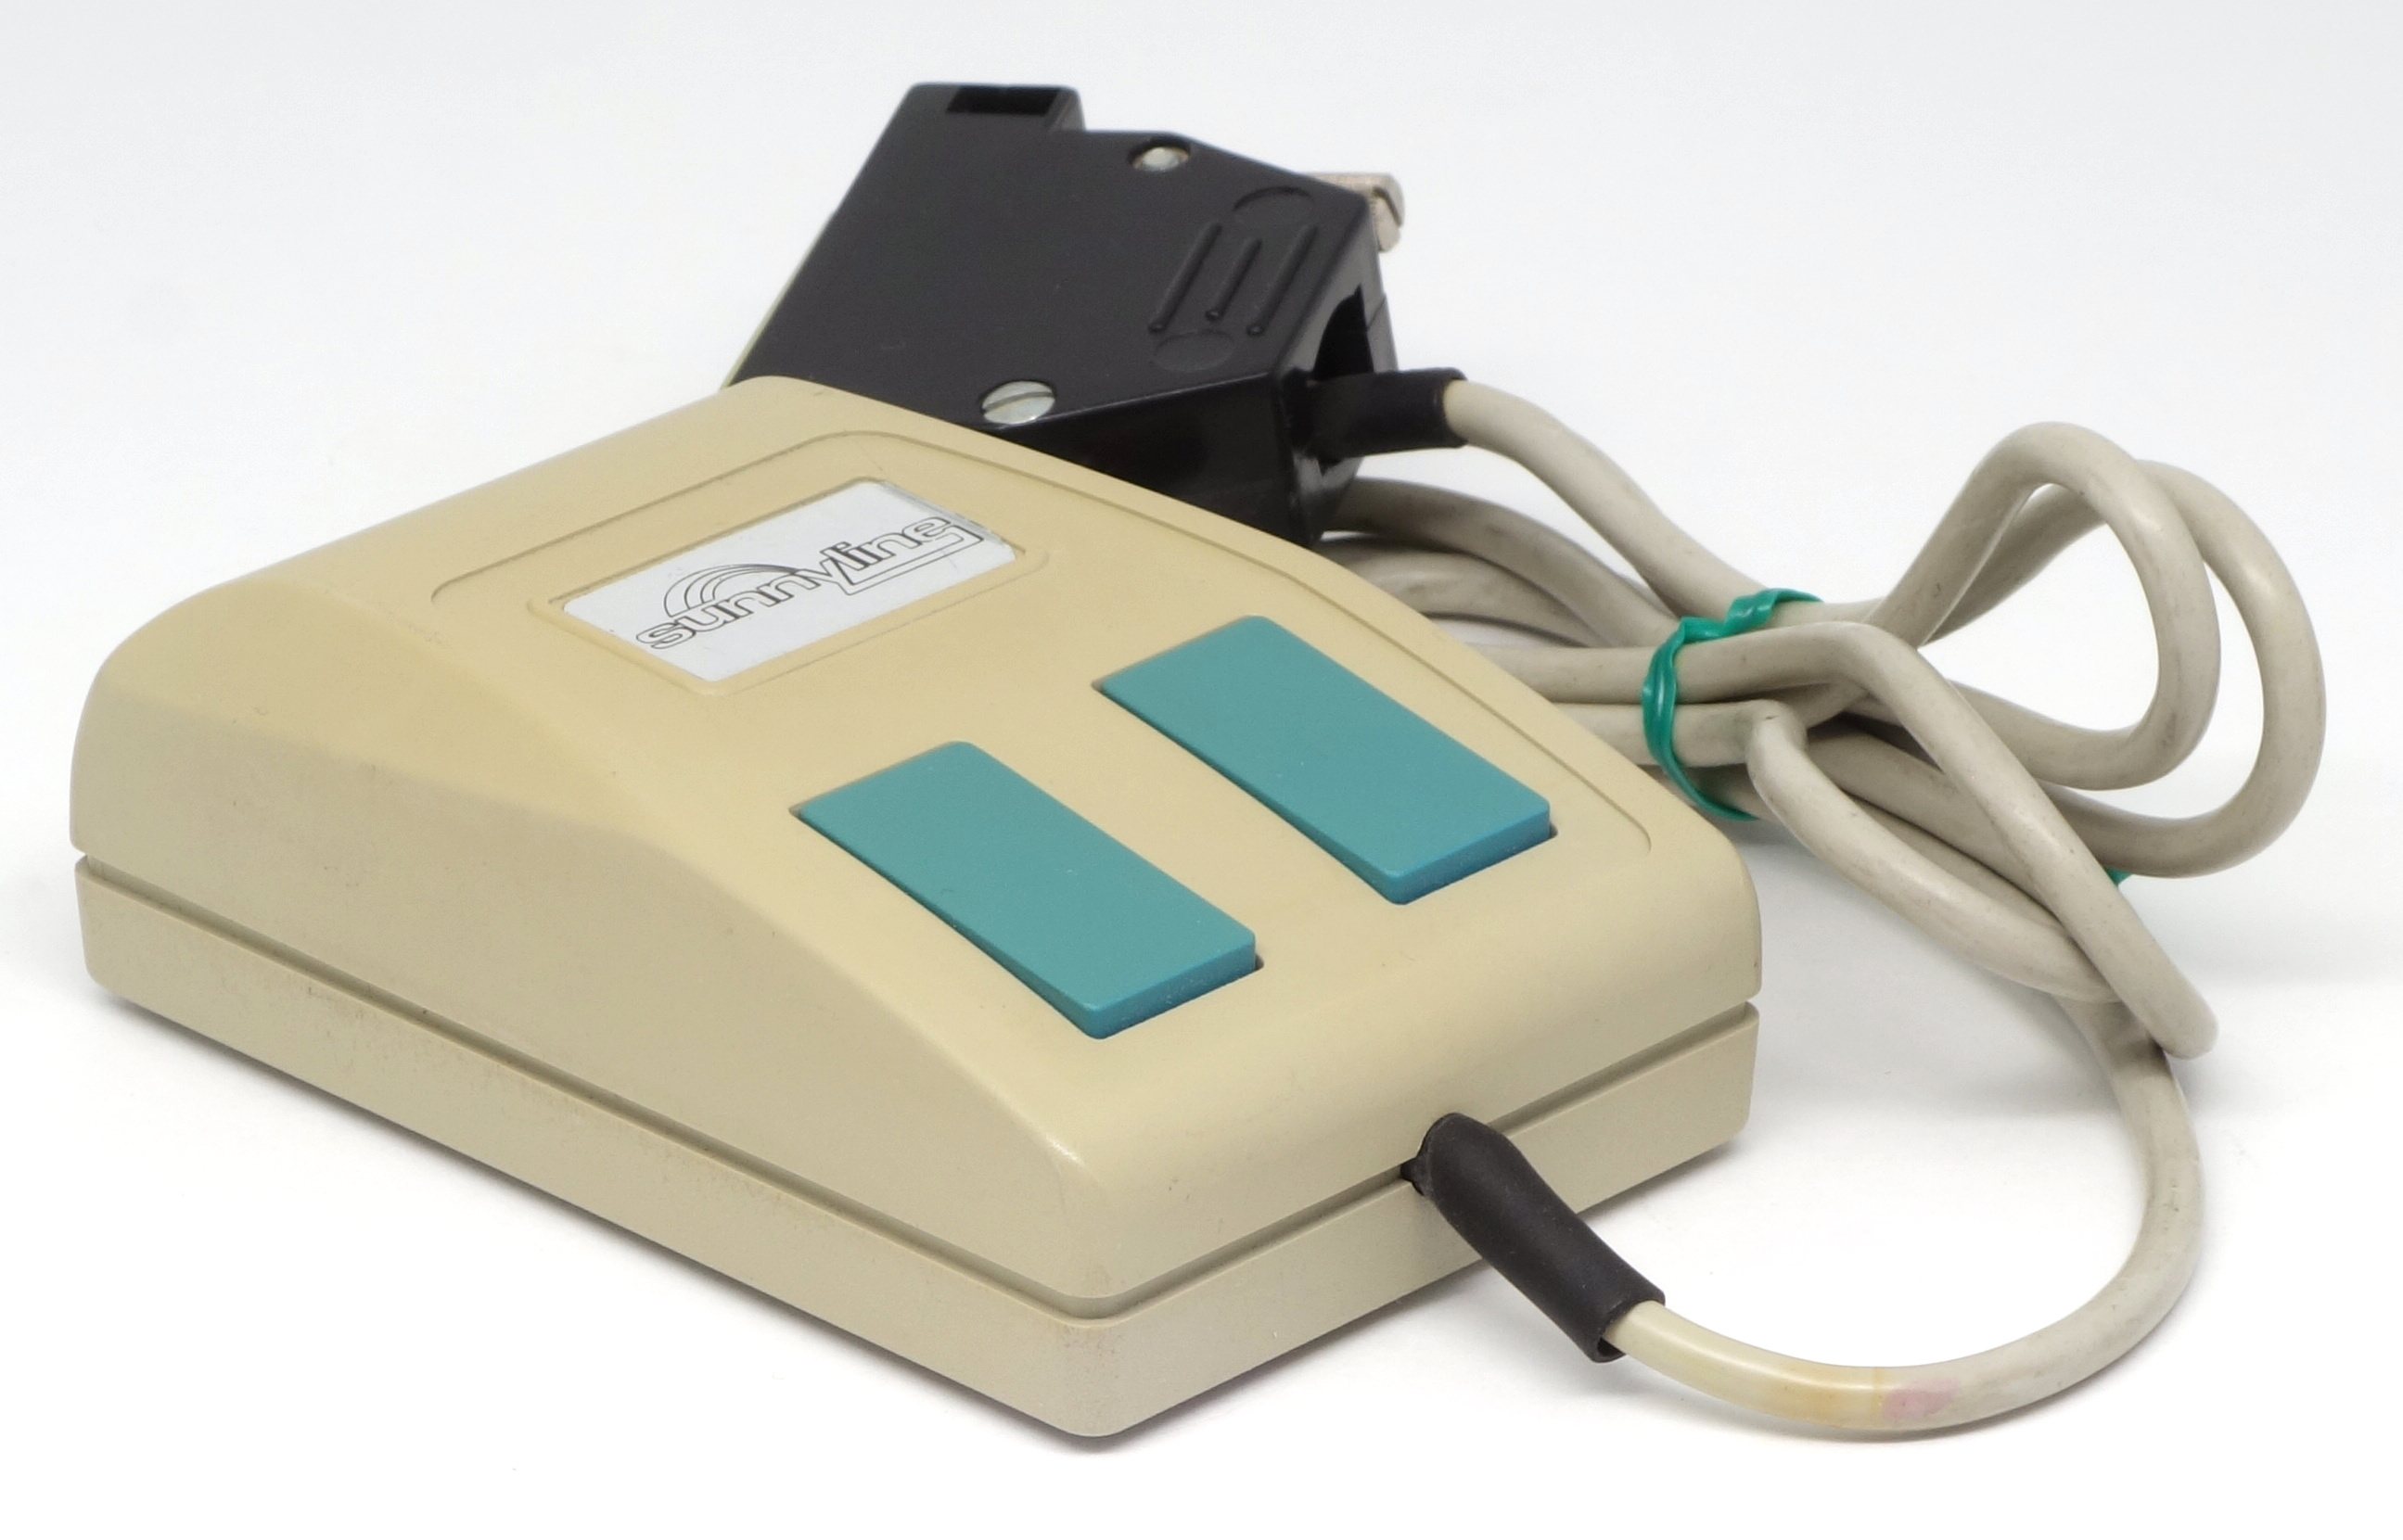
\includegraphics[scale=0.8]{1986_sunnyline_digimouse/pic_30.jpg}
    \caption{DIGIMOUSE}
    \label{fig:SunnylineDIGIMOUSEPic}
\end{figure}

As a result, the mouse received a unique upper part of the body, while the lower part (Fig. \ref{fig:SunnylineDIGIMOUSETopAndBottom}) is almost identical to the 2nd generation AMX mouse released by Depraz in the same 1986.
The bottom of both models demonstrates a number of elements that originally appeared in the Depraz Digimouse P1000 mouse: a ball made of polymer material, a screw-secured removable ring for cleaning the mouse, and mechanical protection of the cable on its exit from the mouse body. A sticker on the underside of the Sunnyline mouse contains information about its Swiss origin, as well as the model name <<DIGIMOUSE D 86 S>>. Although any review or advertising publications about this model are unknown, the assumption that the model number is based on its year of manufacture, as well as the fact that Sunnyline MultiMedia Products AG was founded in 1986 \cite{Sunnyline}, allows us to consider this model to be the first mouse from Sunnyline.

\begin{figure}[h]
    \centering
    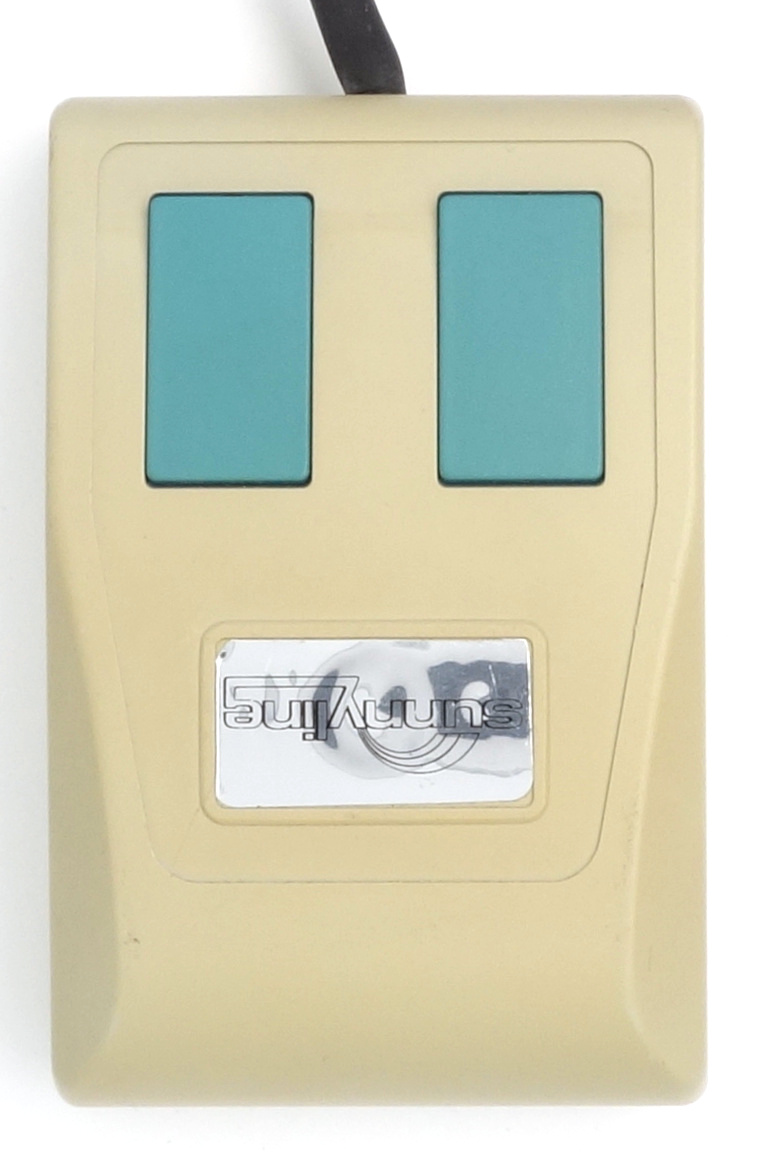
\includegraphics[scale=0.85]{1986_sunnyline_digimouse/top_30.jpg}
    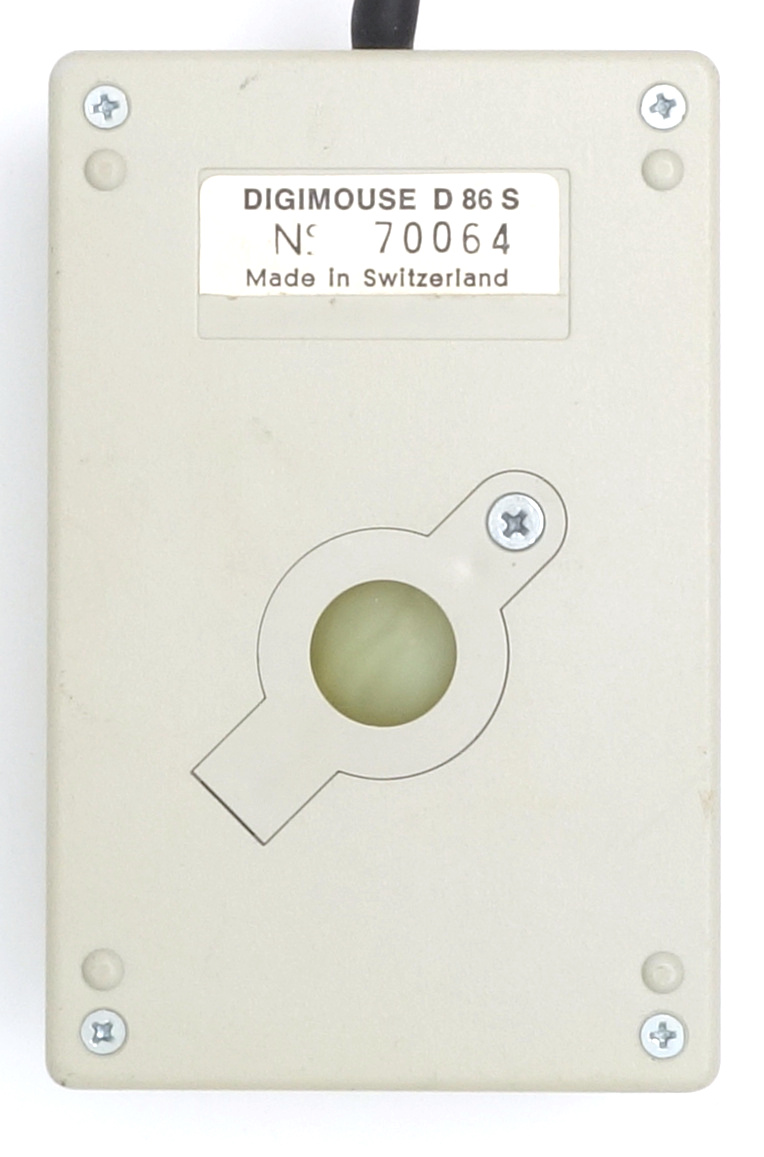
\includegraphics[scale=0.85]{1986_sunnyline_digimouse/bottom_30.jpg}
    \caption{DIGIMOUSE, top and bottom views}
    \label{fig:SunnylineDIGIMOUSETopAndBottom}
\end{figure}

Unlike its close relative - the AMX mouse for BBC Micro computers - the Sunnyline DIGIMOUSE has only two buttons, not three (Fig. \ref{fig:SunnylineDIGIMOUSETopAndBottom}) and a beige body that fits into the dimensions of the AMX mouse, but is improved with beveled edges and rounding at the wrist area. There is a metal plate with the Sunnyline emblem on the upper side, as well as contrasting green buttons. Obviously, the buttons refer to the color scheme of Microsoft's first mouse, released three years earlier and known as the ``Green-Eyed Mouse'', so technically Sunnyline DIGIMOUSE could have been known as the ``Green-Eyed Sunnyline Mouse'' had it been released in more prominent quantities.
In subsequent models, Sunnyline followed a more economical approach, using off-the-shelf body designs from manufacturers without significant modifications.

\begin{figure}[h]
    \centering
    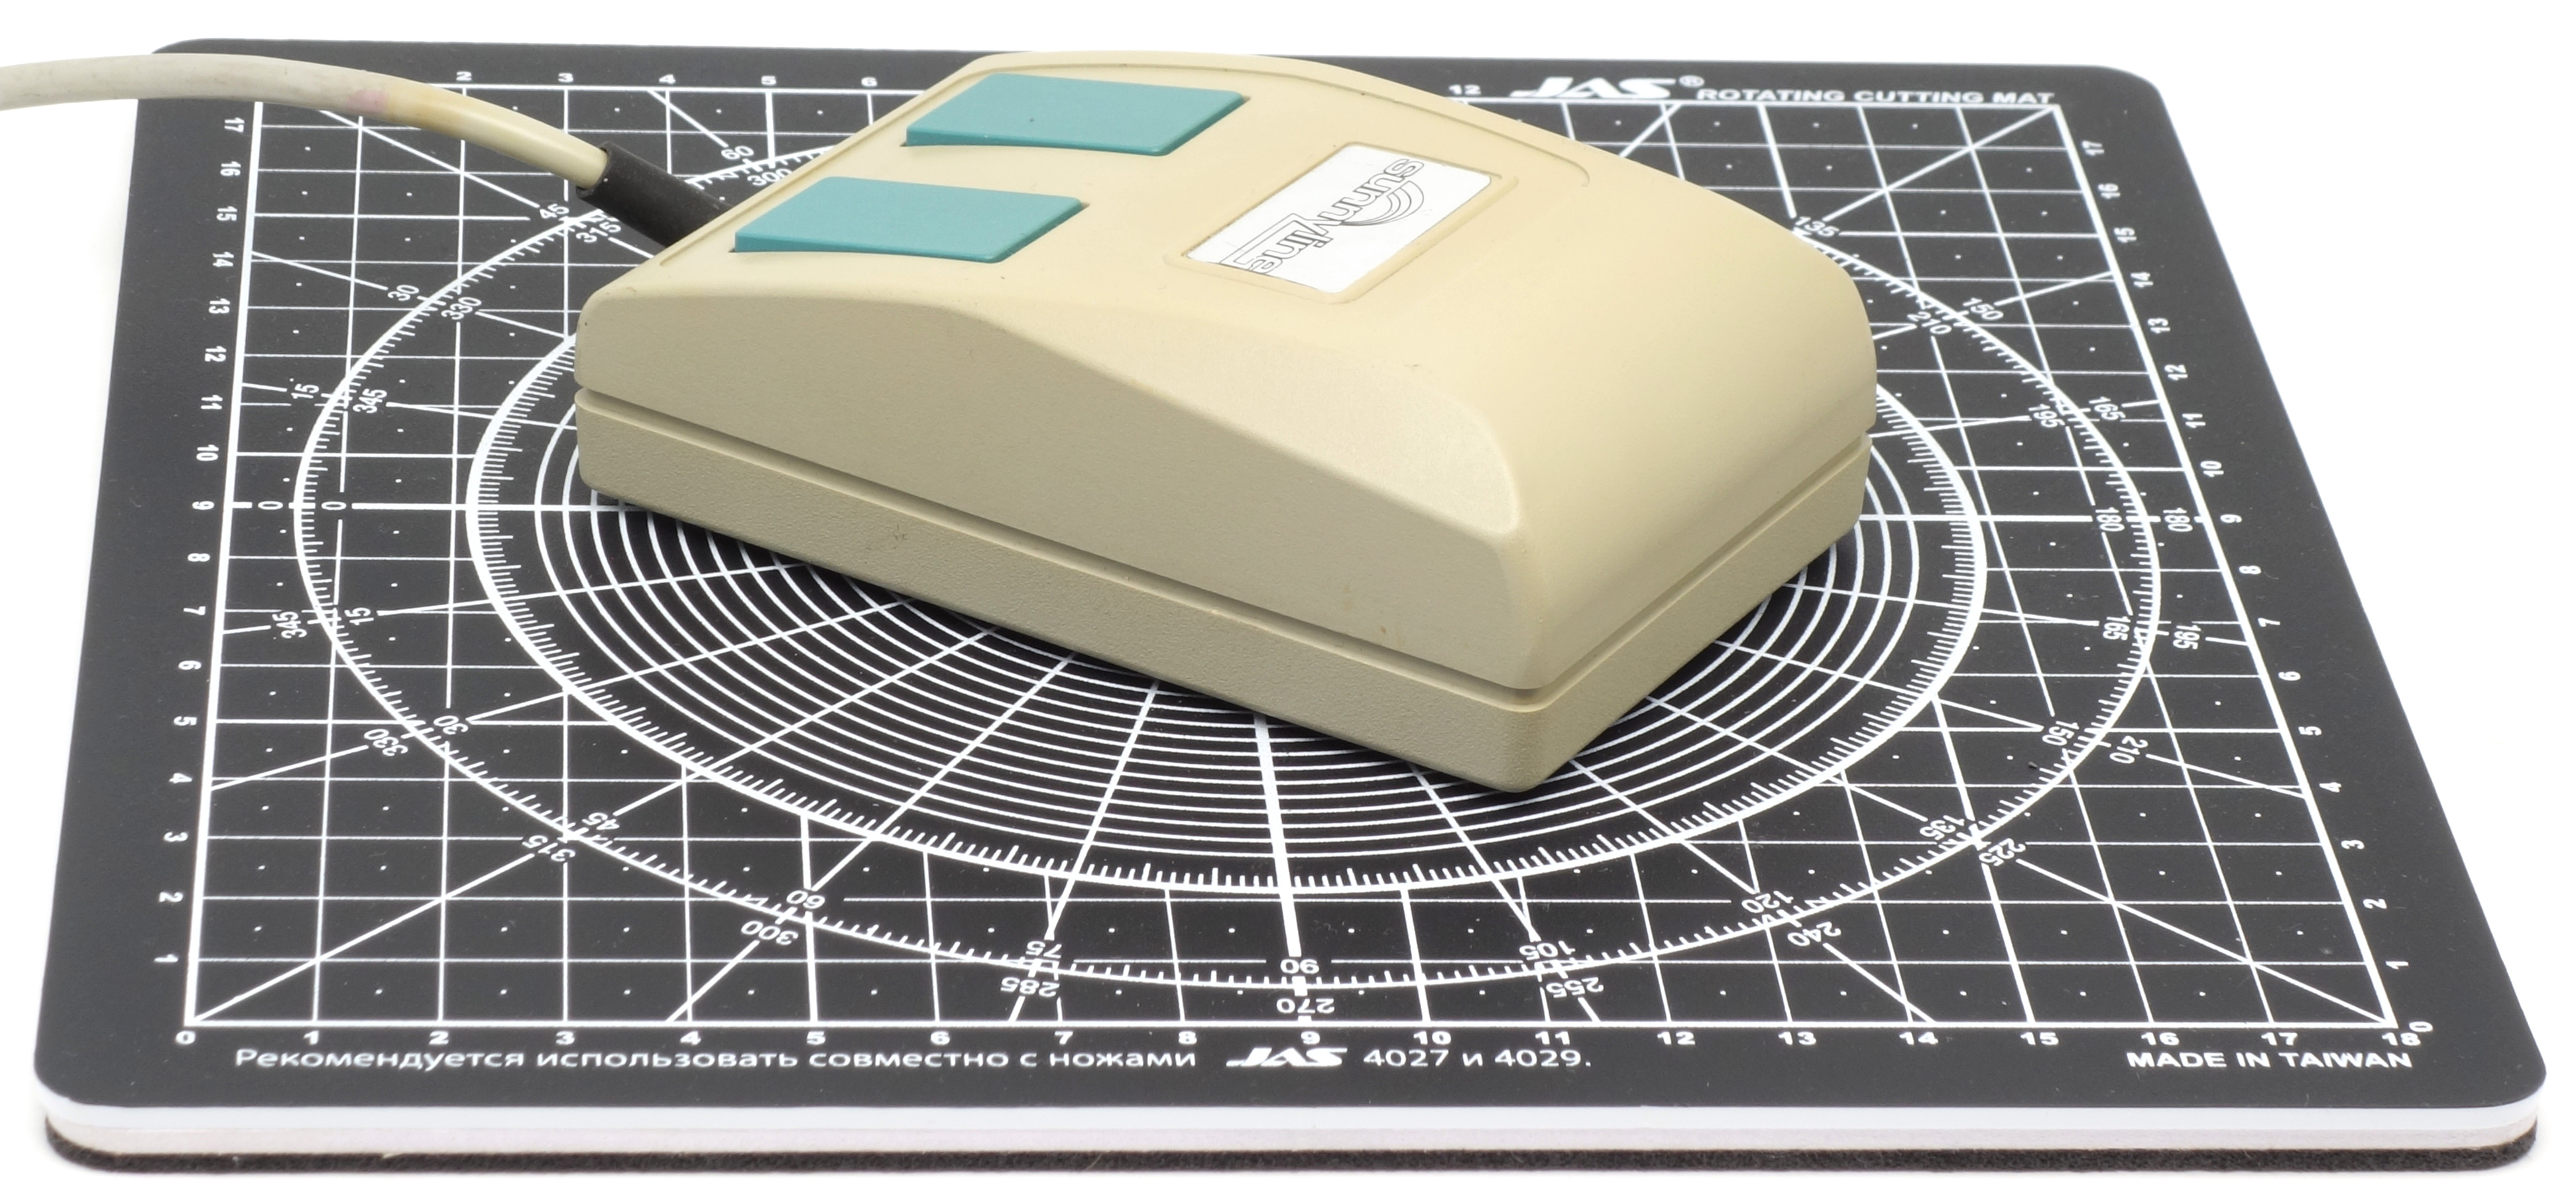
\includegraphics[scale=0.6]{1986_sunnyline_digimouse/size_30.jpg}
    \caption{DIGIMOUSE on a graduated pad with a grid step of 1~cm}
    \label{fig:SunnylineDIGIMOUSESize}
\end{figure}

The mouse has a typical size for mice of the 1980s (figure \ref{fig:SunnylineDIGIMOUSESize}).

\begin{figure}[h]
    \centering
    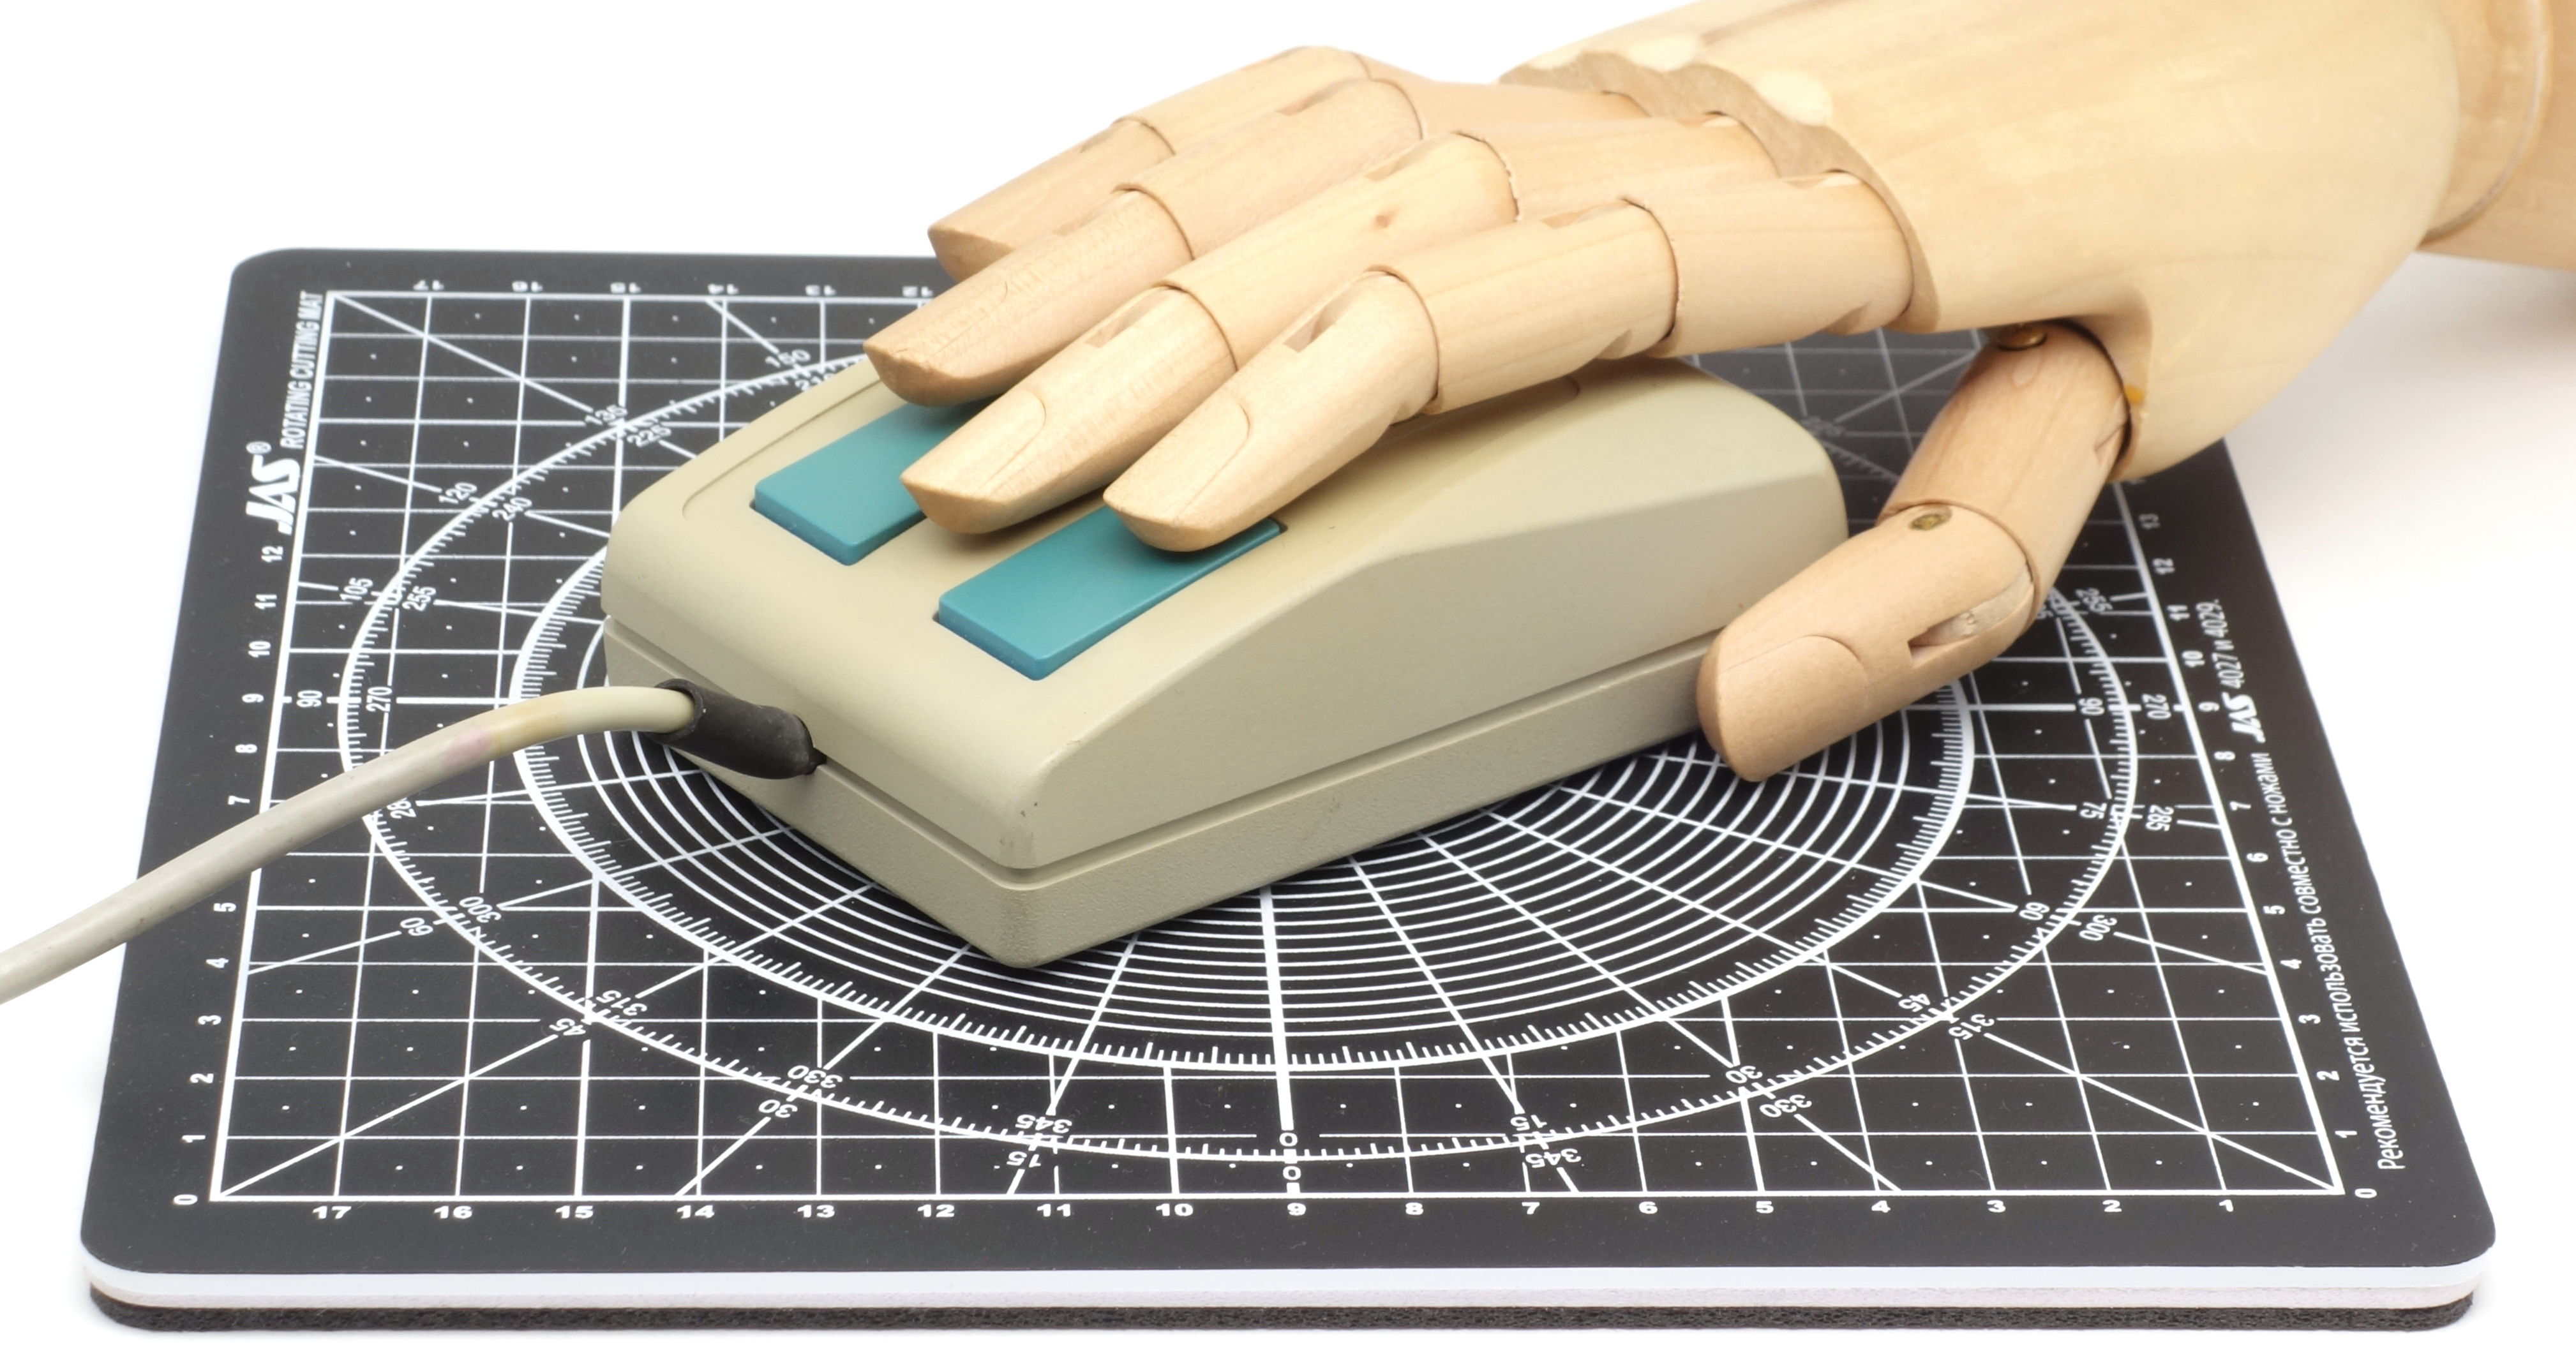
\includegraphics[scale=0.58]{1986_sunnyline_digimouse/hand_30.jpg}
    \caption{DIGIMOUSE with a human hand model}
    \label{fig:SunnylineDIGIMOUSEHand}
\end{figure}

The buttons have a fairly large area, which makes them quite comfortable to press with your fingers. Overall, the rounded edges of the body have some positive effects on ergonomics, but the typical shape of mice from the 80s does not provide significant palm support (Fig. \ref{fig:SunnylineDIGIMOUSEHand}).

 \begin{figure}[h]
    \centering
    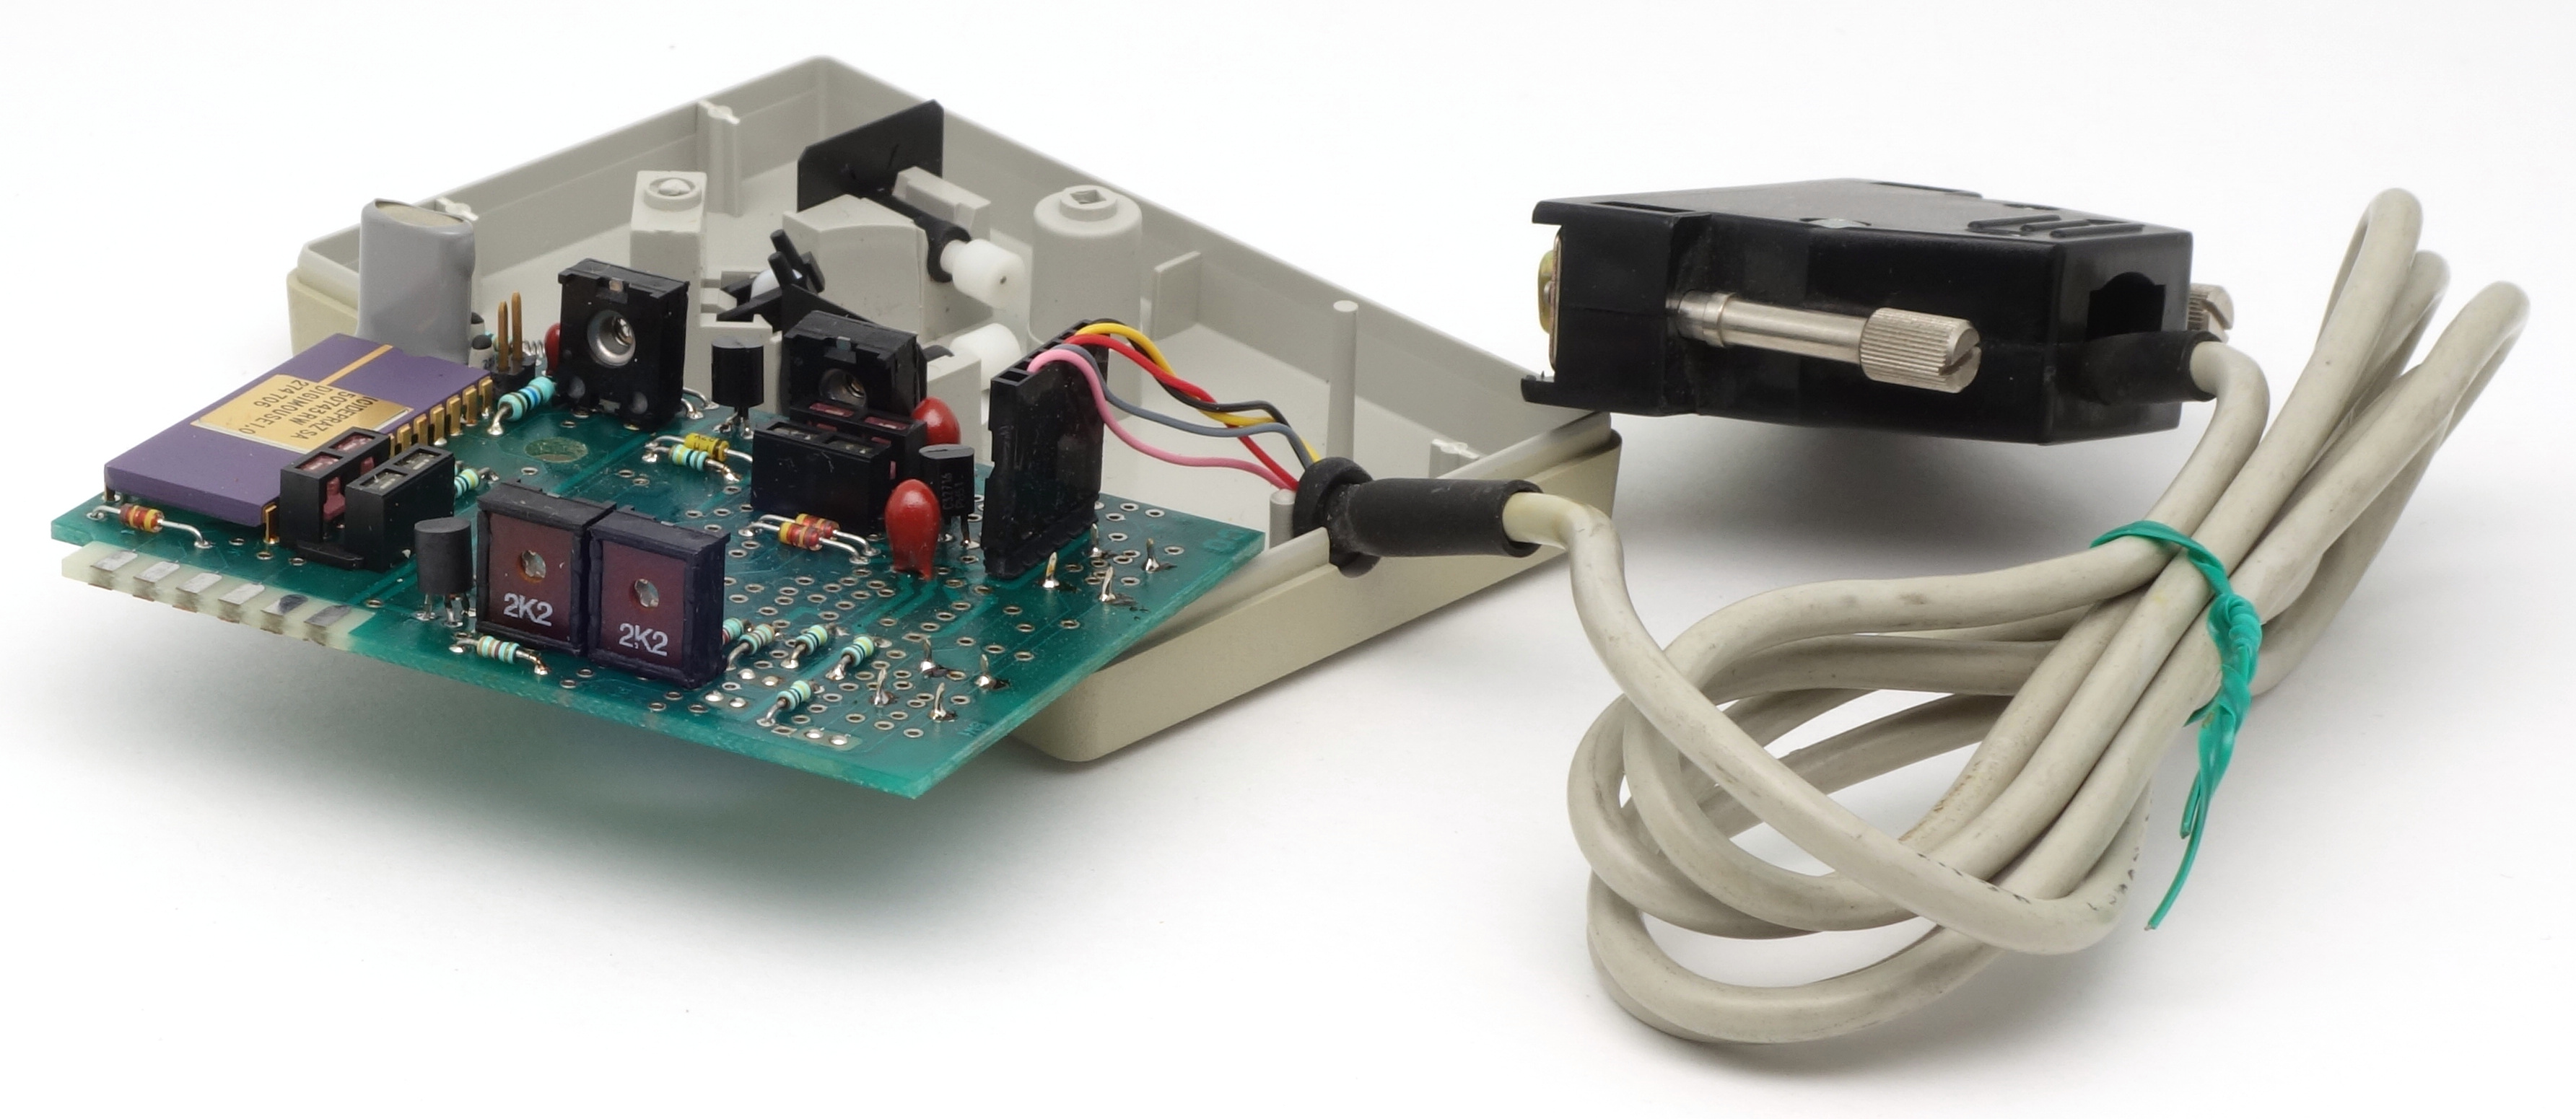
\includegraphics[scale=0.65]{1986_sunnyline_digimouse/inside_30.jpg}
    \caption{DIGIMOUSE disassembled}
    \label{fig:SunnylineDIGIMOUSEInside}
\end{figure}

The internal structure of the mouse is shown in figure \ref{fig:SunnylineDIGIMOUSEInside}. The mouse uses optomechanical encoders and typical Depraz design features: an upside-down printed circuit board, four trimmer resistors for manual adjustment of optocouplers (albeit in atypical rectangular housings), mechanical assemblies mounted on the bottom of the housing, and the optical interrupter disk equipped with a fixed mask that reduces the light exposure area. Unlike earlier Depraz models, the disk is made not of metal, but of plastic (like the AMX mouse of the same year). Also worthy of mention is the characteristic-looking microprocessor with a copyright from Depraz and the text ``DIGIMOUSE 1.0''. This chip, added to the design of the Depraz quadrature mice by Ren\'e Sommer, is a Motorola 6805 microcontroller that provides communication between the mouse and the computer via the RS-232 interface. The variety of Depraz Digimoue mice that contained it is the world's first microprocessor-based \cite{smaky} mouse. However, the Sunnyline DIGIMOUSE, released a few years later, differs from Sommer's solution in that it does not have an external power source thanks to more energy-efficient LEDs, which became available in 1986.

\begin{thebibliography}{9}
\bibitem {Sunnyline} Sunnyline MultiMedia Products AG, Mouse \& Keyboards, Mouse, Germany. Company List, Suppliers, Distributors, Importers, Exporters, Dealers, Manufacturers \url{https://www.companiess.com/sunnyline_multimedia_products_ag_info1208463.html}
\bibitem {smaky} smaky.ch - Une histoire de l'informatique en Suisse. Chapitre 7 - Histoire de la souris \url{https://web.archive.org/web/20211019022335/http://www.smaky.ch/chapitre.php?id=lami_7}
\end{thebibliography}
\end{document}
